\documentclass[../ClipsManualeUtente.tex]{subfiles}

\begin{document}
\section{Per iniziare: Navigazione indoor}
	Per iniziare ad utilizzare subito l'applicazione e navigare nell'edificio di tuo interesse:
	\begin{enumerate}
		\item attiva il \textbf{bluetooth}. Altrimenti all'avvio l'applicazione ti chiederà il permesso di attivarlo (figura \ref{fig:AvvisoBLE});
		\item attiva una \textbf{connessione dati} oppure una \textbf{connessione Wi-fi} e assicurati che lo smartphone sia connesso ad Internet. Se si avvierà l'applicazione senza una connessione Internet attiva l'applicazione segnalerà che la corretta navigazione non è garantita.
		\item \textbf{avvia l'applicazione} selezionando l'icona 
\includegraphics[scale=0.4]{img/LogoApp};
		\item assicurati di essere in un \textbf{edifico supportato} dall'applicazione. Per assicurarsi di ciò basta accertarsi che dalla schermata principale dell'applicazione siano visibili le informazioni dell'edificio;
		
		\begin{framed}
			\textbf{Nota:} solo per i dispositivi con \textbf{Android `Marshmallow' 6.0} - il \textbf{GPS} dello smartphone deve essere \textbf{attivato} prima di avviare l'applicazione. Se non è attivo, all'avvio, l'applicazione chiederà il permesso di attivarlo come mostrato in figura \ref{fig:AvvisoGPS}.
		\end{framed}
		
		\item nella schermata principale (figura \ref{fig:HomeApp}), se l'edificio è stato identificato, potrai trovare:
		\begin{itemize}
			\item informazioni relative all'edificio: nome, indirizzo e una breve descrizione dell'edificio;
			\item orari di apertura e chiusura dell'edificio;
			\item una lista di categorie che raccolgono tutte le possibili aree d'interesse da raggiungere;
		\end{itemize}
		\item dalla lista sotto: \textit{`La Struttura'} mostrata in figura \ref{fig:CategoriePoi} seleziona la categoria di tuo interesse;
		
		\begin{figure} [p]
			\centering
			\subfloat[][Avviso mostrato nel caso il Bluetooth sia spento]
			{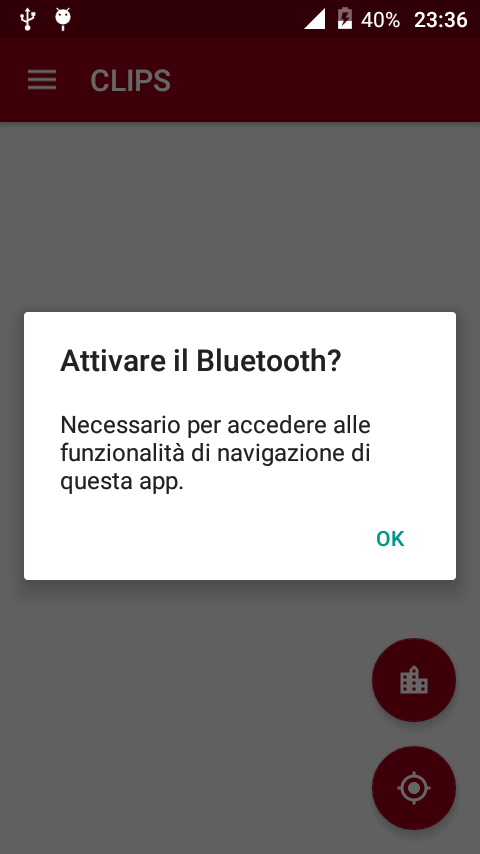
\includegraphics[width=.33\textwidth]{img2/Home-AttivaBluetooth}
			\label{fig:AvvisoBLE}} \quad
			\hspace{1.5cm}
			\subfloat[][Avviso mostrato nel caso il servizio di geolocalizzazione sia spento]
			{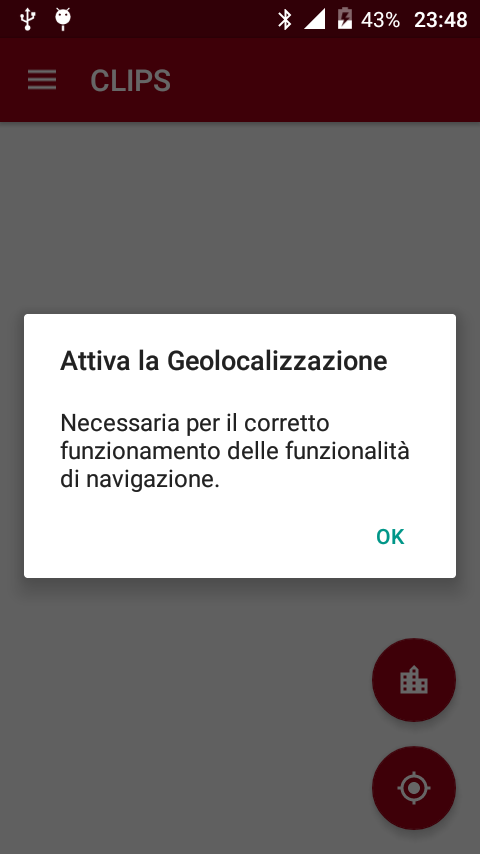
\includegraphics[width=.33\textwidth]{img2/Home-AttivaGeolocalizzazione}
			\label{fig:AvvisoGPS}} \\
			
			\subfloat[][Schermata principale con informazioni dell'edificio rilevato]
			{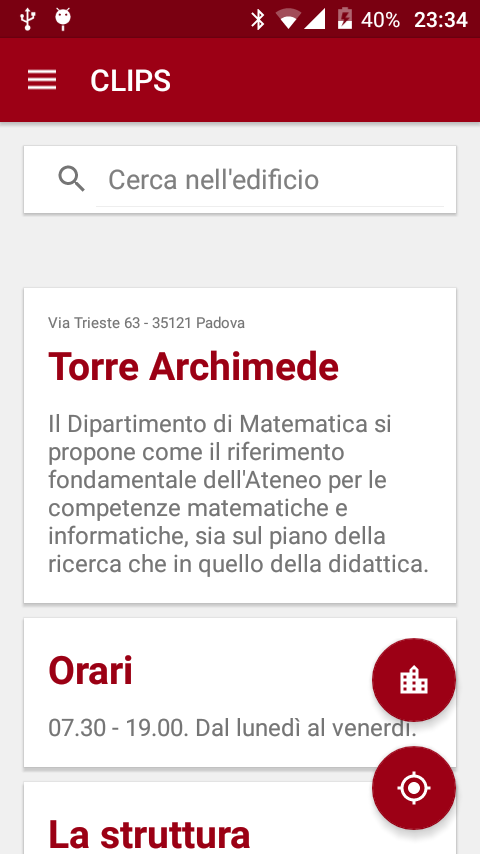
\includegraphics[width=.33\textwidth]{img2/Home-EdificioCaricato}
			\label{fig:HomeApp}} \quad
			\hspace{1.5cm}
			\subfloat[][Lista di categorie delle possibili destinazioni]
			{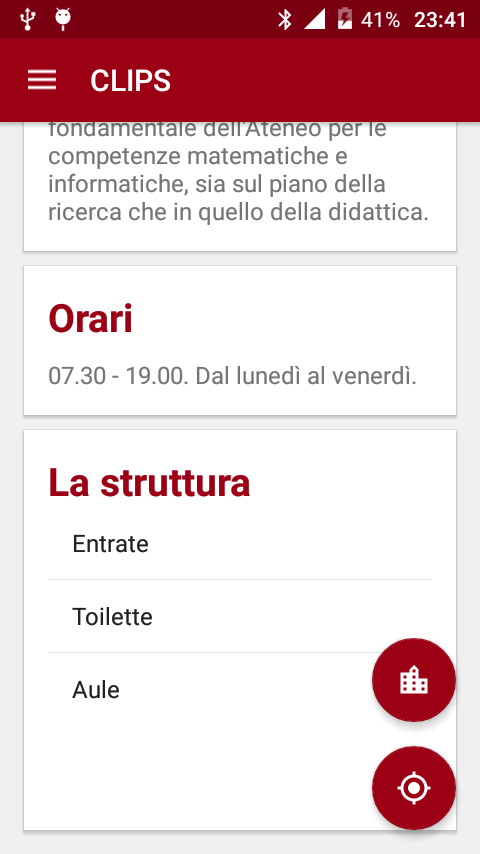
\includegraphics[width=.33\textwidth]{img2/Home-EdificioCaricatoCategorie}
			\label{fig:CategoriePoi}} \\
			\caption{Avvisi mostrati all'avvio dell'applicazione e Schermata principale dell'applicazione}
		\end{figure}
			
			
		\newpage	
		
		\item si aprirà una schermata simile a quella in figura \ref{fig:ListaPoi}, ora puoi selezionare l'area d'interesse che vuoi raggiungere;
		\item segui l'indicazione evidenziata per raggiungere la prossima area e continua così fino ad arrivare alla destinazione scelta (figura \ref{fig:ListaIstruzioni});
		\item se si dovesse sbagliare direzione l'applicazione lo segnalerà richiedendo un ricalcolo del percorso \ref{fig:AvvioRicalcoloPercorso};
		\item nel caso avessi bisogno di più informazioni, seleziona una singola istruzione, si aprirà la schermata come in figura \ref{fig:DettaglioIstruzione};
		\item seleziona una foto per visualizzarla meglio come in figura \ref{fig:VisioneFotoIstruzione}.			
				
	\end{enumerate}

	\vfill		
		
		\begin{figure} [h]
			\centering
			\subfloat[][Lista delle possibili destinazioni della categoria \textit{`Aule'}]
			{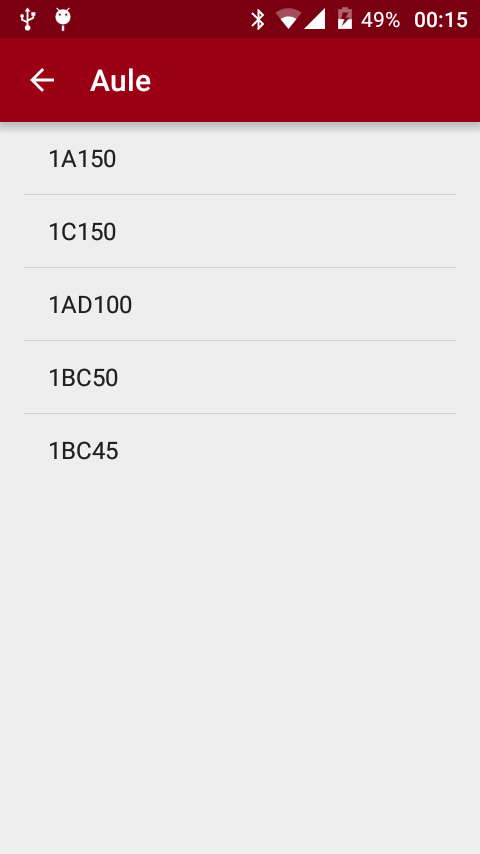
\includegraphics[width=.33\textwidth]{img2/Navigazione-DestinazioniCategoria}
			\label{fig:ListaPoi}} \quad
			\hspace{1.5cm}
			\subfloat[][Lista di istruzioni da seguire per raggiungere la destinazione scelta]
			{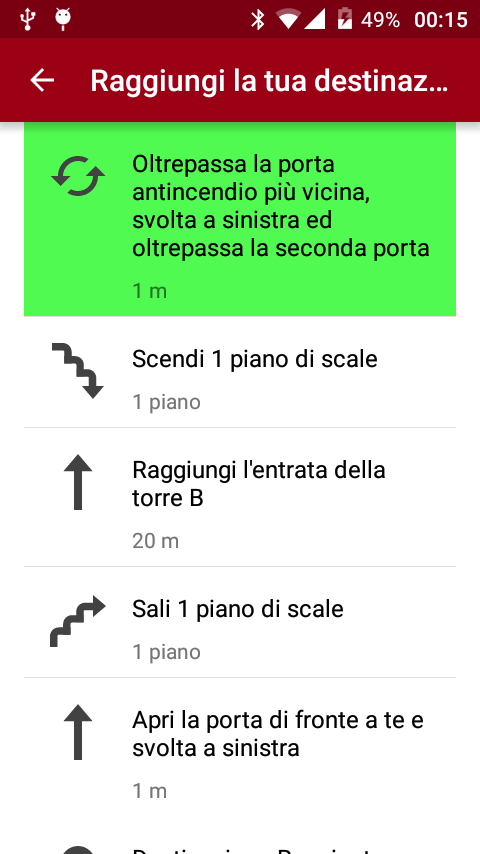
\includegraphics[width=.33\textwidth]{img2/Navigazione-ListaIstruzioni}
			\label{fig:ListaIstruzioni}} \\
			\caption{Cominciare una navigazione}
		\end{figure}
	
	\vfill		
		
	%\newpage	
		
		\begin{figure} [p]
			\centering
			\subfloat[][Avviso percorso seguito errato e richiesta di ricalcolarlo]
			{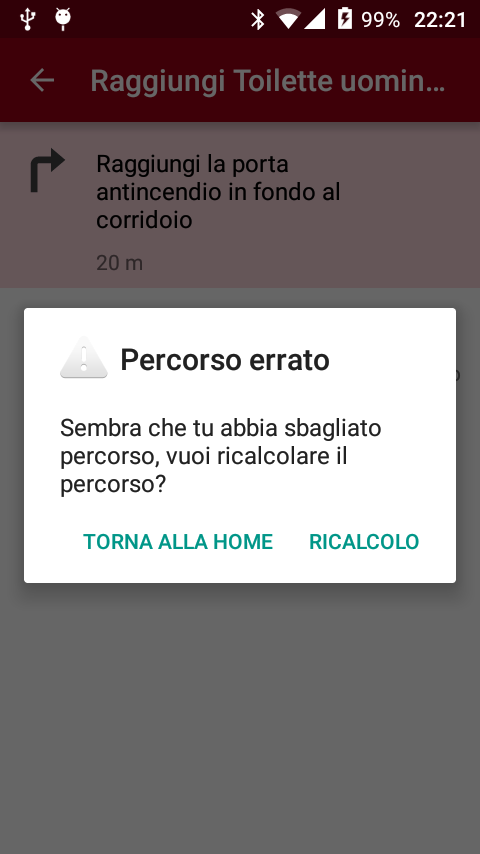
\includegraphics[width=.33\textwidth]{img2/Navigazione-AvvisoRicalcoloPercorso}
			\label{fig:AvvisoRicalcoloPercorso}} \quad
			\hspace{1.5cm}
			\subfloat[][Dettaglio istruzione selezionata]
			{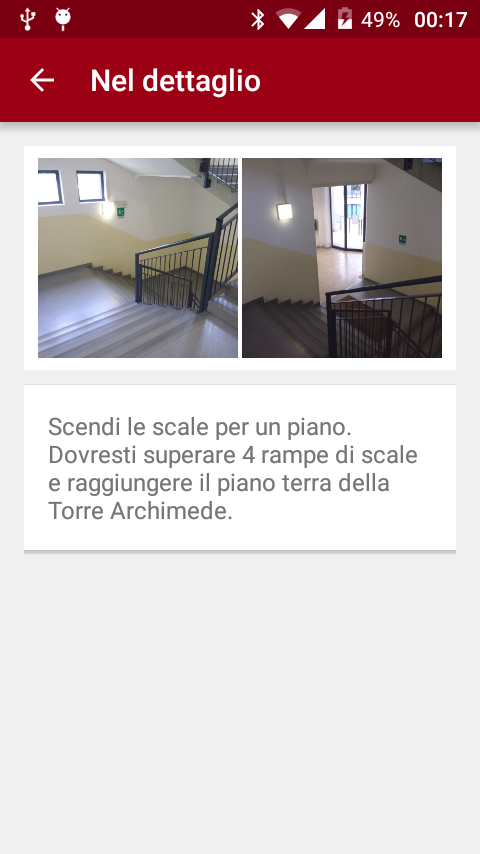
\includegraphics[width=.33\textwidth]{img2/Navigazione-DettaglioIstruzione}
			\label{fig:DettaglioIstruzione}} \\
			
			\subfloat[][Visione della foto dell'istruzione selezionata]
			{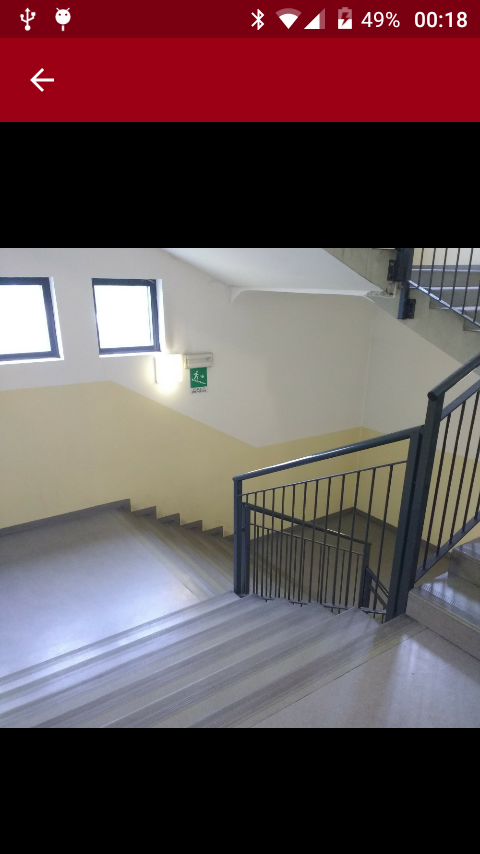
\includegraphics[width=.33\textwidth]{img2/Navigazione-VisioneFotoIstruzione}
			\label{fig:VisioneFotoIstruzione}} \\		
			\caption{Approfondire le istruzioni di una navigazione}			
		\end{figure}		
	

\end{document}